%\documentclass[a4paper]{scrartcl}
\documentclass[a4paper]{article}
\usepackage{fullpage}
\usepackage{setspace}
\usepackage{url}
\usepackage{mdwlist}
\usepackage{polski}
\usepackage[utf8x]{inputenc}
\usepackage{color}
\usepackage{mathtools}
\usepackage{graphicx}
\usepackage[unicode=true]{hyperref}
\usepackage{multirow}
\usepackage[table]{xcolor}
\usepackage{subfig}
\usepackage{listings}
\newcommand{\HRule}{\rule{\linewidth}{0.5mm}}

\lstset{ %
basicstyle=\footnotesize,       % the size of the fonts that are used for the code
numbers=left,                   % where to put the line\dywiz numbers
numberstyle=\footnotesize,      % the size of the fonts that are used for the line\dywiz numbers
stepnumber=2,                   % the step between two line\dywiz numbers. If it's 1, each line 
% will be numbered
numbersep=5pt,                  % how far the line\dywiz numbers are from the code
frame=single,                   % adds a~frame around the code
}

\begin{document}
\begin{titlepage}
  
  \begin{center}
    
    
    % Upper part of the page
    
\includegraphics[width=0.3\textwidth]{logo.jpg}\\[1cm]    
    
    \begin{onehalfspace}
    \textsc{\LARGE Wydział Elektryczny Politechniki Warszawskiej}\\[1.5cm]
    \end{onehalfspace}
    

    
    \textsc{\Large Grafika Komputerowa}\\[0.5cm]
    
    
    % Title
    \HRule \\[0.4cm]
    { \huge \bfseries Coffeecam - wirtualna kamera}\\[0.2cm]
    \HRule \\[1.5cm]
    
    % Author and supervisor
      \begin{flushleft} \large
        \emph{Autorzy:}\\
        Bartosz \textsc{Pieńkowski} \\
        Barnaba \textsc{Turek}
      \end{flushleft}
    \vfill
    
    % Bottom of the page
    {\large \today}
    
  \end{center}
  
\end{titlepage}
\sloppy

\abstract{
Celem serii projektów z~przedmiotu Grafika Komputerowa jest utworzenie prostego silnika graficznego 
(i~zapoznanie się od strony graficznej z~podstawowymi zadaniami grafiki komputerowej, takimi jak rzutowanie,
eliminacja elementów zasłoniętych i~cieniowanie). 

Zdecydowaliśmy się zaimplementować projekt w~języku coffeescript.

Pierwsza część projektu polega na utworzeniu wirtualnej kamery. Kamera ma obsługiwać zmianę pozycji, ogniskowej i~kąta, w~którym jest skierowana.
Druga część projektu polegała na dodaniu algorytmu zasłaniania obiektów. Zastosowaliśmy Algorytm malarski.
W~trzeciej części projektu dodaliśmy cieniowanie metodą Blinna-Phonga.

\begin{figure}[p!]
  \caption{Struktura projektu}
  \centering
  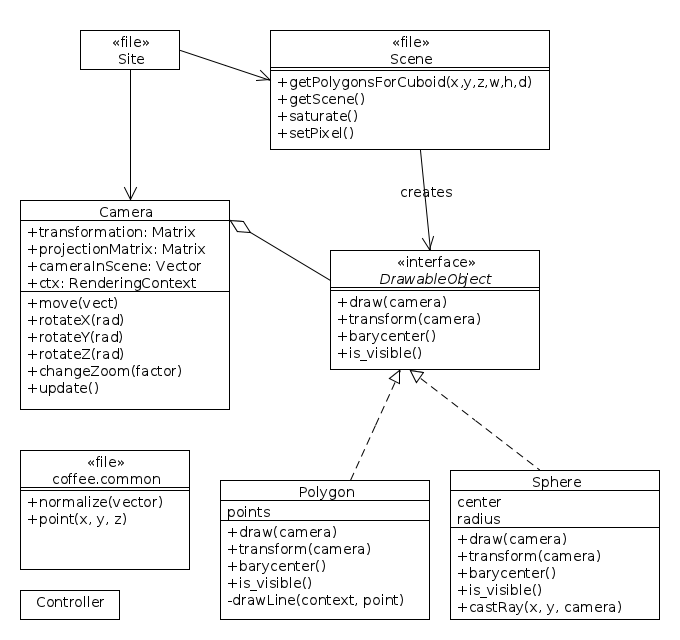
\includegraphics[width=\textwidth]{coffeecam_uml.png}
  \label{uml}
\end{figure}


\section{Wirtualna kamera}
\subsection{Struktura projektu}

Projekt podzielony jest na pliki .coffee, z~których każdy zostaje skomplikowany do pliku .js (javascript).
Zawartość każdego pliku wynikowego jest opakowana w~anonimową funkcję, aby zniwelować ryzyko konfliktu nazw z~innymi skryptami.

Zmienne i~funkcje potrzebne do komunikacji pomiędzy modułami dostępne są za pomocą globalnej zmiennej coffecam.

Nie wszystkie obiekty przedstawione na diagramie \ref{uml} są w~istocie klasami - z~wyjątkiem klas 
\textbf{Camera}, \textbf{Controller}, \textbf{Polygon}, \textbf{Sphere}.
nie potrzebowaliśmy przechowywać żadnego stanu, a~tylko logicznie podzielić udostępniane funkcje.
\begin{description}
  \item[camera.coffee] W~tym pliku zdefiniowana jest klasa \textbf{Camera}. Obiekty tej klasy reprezentują wirtualną kamerę.
    Udostępniają takie metody jak \textbf{move()}, \textbf{rotateX()}, \textbf{rotateY()}, \textbf{rotateZ()}, \textbf{update()}.
    Stanem, przechowywanym przez obiekty tej klasy jest np. transformacja potrzebna do zamienienia koordynatów z~układu współrzędnych sceny na układ współrzędnych kamery. Ponadto obiekty tej klasy przechowują informacje i~udostępniają metody dotyczące źródła światła.
  \item[common.coffee] W~tym pliku zawierają się funkcje pomocnicze, używane w~pozostałych plikach, takie jak \textbf{normalize} i~\textbf{point}.
  \item[controller.coffee] obiekt tej klasy reprezentuje kontroler użytkownika.
    Pozwala on w~przejrzysty sposób powiązać zdarzenia związane z~wciskaniem przez użytkownika klawiszy z~odpowiadającymi im akcjami.
  \item[scene.coffee] W~tym pliku zdefiniowane są obiekty, które możemy narysować, takie jak \textbf{Polygon} i~\textbf{Sphere}.
    Obiekty te reprezentują wspólny, prosty interfejs złożony z~metod \textbf{draw()} i~\textbf{transform()}.
    Plik udostępnia także funkcje pozwalające w~czytelny sposób zbudować prostopadłościan z~wielokątów, oraz funkcje odpowiadające za konstrukcję sceny.
  \item[site.coffee] Plik odpowiada za połączenie pozostałych plików, inicjalizacje potrzebnych obiektów i~zapewnienie im zależności (zgodnie ze wzorcem \emph{dependency injection}.
\end{description}

\subsection{Działanie kamery}
Obiekt kamery przechowuje macierz transformacji, początkowo ustawioną na macierz jednostkową (z~dokładnością do znaku, ze względu na skrętności układów)\cite{openGL}.
Macierz transformacji obliczana jest na nowo po każdym ruchu kamery. Obliczenie nowej macierzy polega na pomnożeniu aktualnej macierzy przez żądaną transformacje.

W~pliku kamery stworzone są funkcje pomocnicze, pozwalające wyliczyć macierz konkretnej transformacji.
Zastosowaliśmy wzorzec projektowy \emph{dekorator}, aby dodać do funkcji obliczających macierze inne zachowania --
i~w~rezultacie otrzymać metory pozwalające faktycznie poruszyć kamerą.

Te zachowania to pomnożenie aktualnej macierzy translacji przez dekorowaną macierz, obliczenie nowej pozycji kamery w~koordynatach sceny (co przyspiesza działanie algorytmu malarskiego) oraz obliczenie położenia źródła światła w~układzie współrzędnych kamery (co przyspiesza działanie algorytmu \emph{Blinna\dywiz Phonga}).
Na końcu dekorator wykonuje funkcję update, co pozwala uprościć obsługę kamery do wywołania jednej funkcji na jedną akcję.

Dostępne transformacje to przesunięcia i~obroty kamery (Transformacje utworzylismy na podstawie wykładu\cite{dasa}).

Po wykonaniu każdej operacji na kamerze wywoływana jest metoda \textbf{update}.
Metoda ta polega przetransformowaniu, posortowaniu pod względem odległości od kamery a~następnie narysowaniu wszystkich elementów na ekranie. 

Macierz transformacji mnożona jest przez macierz rzutowania (Obliczaną kiedy kamera jest tworzona i~przy zmianie ogniskowej)\cite{openGL} tylko raz.
Każda z~rysowanych obiektów sam wie, jak się narysować.
W~przypadku klasy \textbf{Polygon}, która nie wymaga cieniowania, transformacja polega na prostym pomnożeniu wszystkich punktów przez macierz transformacji i~rzutowania.
W~przypadku klasy \textbf{Sphere}, jest to nieco bardziej złożone.
Obliczane są wtedy wszystkie zmienne niezbędne, do narysowania sfery (z~wyjątkiem wartości koloru dla samych punktów).

Na tak przygotowanych obiektach wywoływana jest metoda draw, która rysuje je w~oknie przeglądarki.

\subsection{Scena}
Obiekty, które kamera wyświetla to wielokąty i~sfery.
Wczesne wersje programu obsługiwały tylko wielokąty, stąd rozbudowany sposób budowania sceny (``ulice'' i~``domki'') dotyczy tylko ich.
Sfery zostały dodane w~ostatniej iteracji projektu.
\subsection{Polygon}
Wielokąt to podstawowy obiekt należący do sceny.
Klasa udostępnia z~grubsza ten sam interfejs, co \textbf{Sphere} (różnicą jest konstruktor).
Program zakłada, że kolejne punkty opisujące wielokąt podane są w~sposób uporządkowany.

Wielokąty same w~sobie nie są używane do tworzenia sceny.
Zamiast nich używana jest funkcja, która zwraca od razu tablicę wielokątów, reprezentującą prostopadłościan~-- \textbf{get0olygonsForCuboid} -- pewnego rodzaju fabryka obiektów.

\subsection{Sphere}
Sfera to obiekt dodany w~trzeciej iteracji.
Sfera została dodana, ponieważ jest dużo ciekawszym obiektem do cieniowania niż wielokąt.

Obiekty tej klasy implementują ten sam interfejs, co wielokąty, jednak ich zasada działania jest inna.

Oprócz parametrów opisujących zajmowaną przestrzeń, obiekty tego typu inicjuje się 7 dodatkowymi parametrami.
\begin{description}
  \item[diffusePower] Poziom tego współczynnika opisuje jasność związaną z~rozproszonym odbiciem od sfery.
  \item[spectralPower] Poziom tego współczynnika opisuje jasność związaną z~kierunkowym odbiciem (czyli dotyczy bardziej błyszczących obiektów).
  \item[spectralHardness] Poziom tego współczynnika określa, jak bardzo rozmyte jest odbicie kierunkowe.
    Bardzo wysokie poziomy tego współczynnika powodują, że uzyskujemy przestrzeń bliższą lustru - punktowe źródło światła będzie reprezentowane jako świecący punkt na powierzchni sfery.
  \item[ambientPower] Poziom tego wspólczynnika odpowiada za oświetlenie tła, niezależne od kierunku i~odległości, z~której pada światło (ani od niczego innego.
\end{description}

Pozostałe trzy parametry opisują składowe odpowiadające konkretnym kolorom.

\subsubsection{Cykl renderowania obiektu typu \texttt{Sphere}}
Ponieważ w~naszym przypadku sfery nie są opisane za pomocą wielokątów, tak jak to się najczęściej implementuje, sposób ich renderowania jest nieco bardziej złożony.
Z~drugiej strony rozwiązanie takie pozwoliło nam pominąć proces opisywania sfery za pomocą wielokątów.

Po wywołaniu metody \emph{transform()} przeprowadzany jest szereg transformacji, które przygotowują sferę do rysowania.
Korzystając z~macierzy transformacji i~rzutowania udostępnianych przez obiekt \texttt{Camera}, ustalane są współrzędne środka sfery na rzutni.
Następnie ustalana jest długość promienia po zrzutowaniu.

\begin{figure}[h]
  \centering
  \subfloat[Błyszczący obiekt]{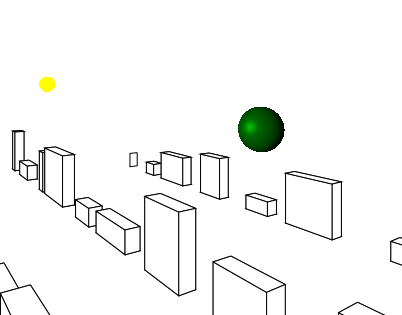
\includegraphics[width=0.3\textwidth]{blyszczacy.png}}                
  \subfloat[Matowy obiekt]{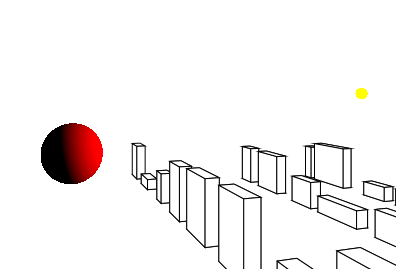
\includegraphics[width=0.3\textwidth]{zwykly.png}}                
  \subfloat[Pod światło]{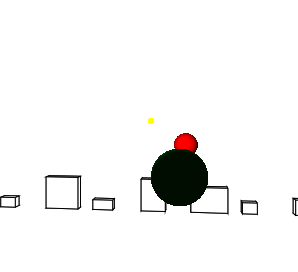
\includegraphics[width=0.3\textwidth]{pod_swiatlo.png}}                
\end{figure}

Za pomocą tych dwóch wartości wyliczany jest prostokąt, określający rysowaną sferę na rzutni.
Współrzedna Z~obu punktów charakterystycznych tego prostokąta określana jest na 1 - współrzędną graniczną, powyżej której rzutowane obiekty sa obcinane (bo znajdują się przed rzutnią).
Po pomnożeniu odwrotności macierzy rzutowania przez uzyskane w~ten sposób punkty uzyskiwane są punkty, które określają współrzędne prostokąta opisującego kulę po rzutowaniu.

Z~wartości współrzednych po zrzutowaniu wiemy też, ile pikseli zajmie rzut sfery na rysowanym obrazie.

Po wywołaniu metody \texttt{draw()}, przechodzimy przez punkt na rzutni odpowiadający każdemu z~poszukiwanych pikseli.
Dla każdego takiego punktu wyznaczamy prostą przechodzącą przez niego i~środek układu współrzędnych (czyli położenie oka kamery).

\begin{figure}[h]
  \centering
  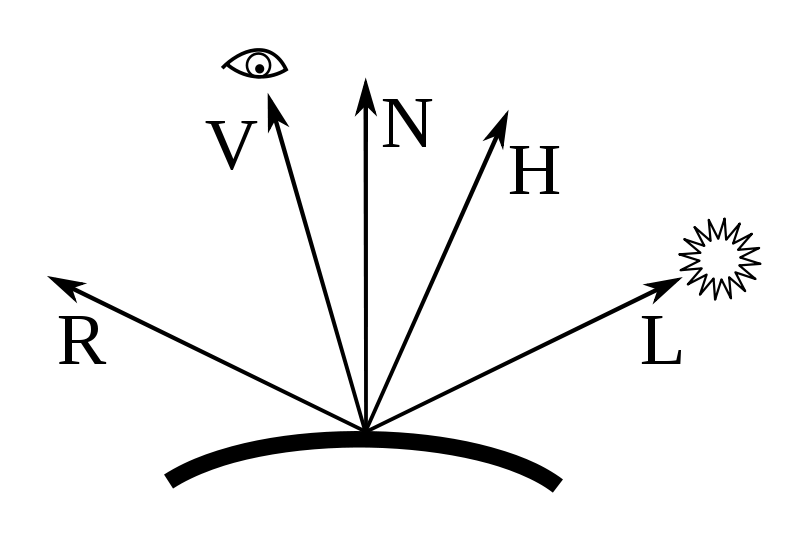
\includegraphics[width=0.28\textwidth]{blinn.png}
  \caption{Wektory biorące udział w obliczeniu jasności punktu w modelu Blinna-Phonga}
\end{figure}

Następnie rozwiązujemy równanie kwadratowe, by znaleźć punkt przecięcia tej prostej ze sferą.
Dla tego punktu obliczane są wektory: normalny (N), kierunku światła (L) i~kierunku patrzenia (V), oraz H, a~na podstawie tych wektorów, zgodnie z~algorytmem cieniowania Blinna\dywiz Phonga wyznaczane są kolory poszczególnych pikseli.

\section{Eliminacja powierzchni zasłoniętych}
Celem drugiego etapu projektu było zaimplementowanie wybranego algorytmu eliminacji powierzchni zasłoniętych.

Ze względu na prostotę sceny zdecydowaliśmy na algorytm malarski.
Działanie tego algorytmu polega na rysowaniu obiektów w~kolejności ustalonej przez ich odległość od kamery.

\subsection{Implementacja}
Algorytm nie zajął zbyt wiele miejsca i~nie uznaliśmy za stosowne dodawać kolejnej klasy do obiektu.
Dodaliśmy kod do klasy \emph{Camera}.

Działanie algorytmu składa się z~trzech kroków.
W~pierwszym kroku obliczamy współrzędne kamery w~układzie odniesienia sceny.

Ponieważ kamera zawsze znajduje się w~punkcie
\[
P_{cam} = 
\begin{bmatrix}
  0 & 0 & 0 & 0 \\
  0 & 0 & 0 & 0 \\
  0 & 0 & 0 & 0 \\
  0 & 0 & 0 & 1
\end{bmatrix}
\]

i~w~każdej klatce zna swoją pozycję względem początku układu współrzędnych sceny (daną macierzą transformacji \texttt{@transformation}), możemy łatwo obliczyć położenie kamery w~układzie współrzędnych sceny.

Transformacja, której szukamy (transformująca położenie z~układu kamery do układu sceny) jest transformacją odwrotną do \texttt{@transformation}, zatem współrzędne kamery w~układzie współrzędnych możemy policzyć w~następujący sposób:
$$
\tt{} P_{cam}^\prime = \tt{@transformation}\tt^{-1} \times P_{cam}
$$

Następnym krokiem jest obliczenie odległości środków ciężkości rysowanych wielokątów od punktu $P_{cam}^\prime$. 
W~tym celu obliczamy środek ciężkości wielokąta \texttt{barycenter}, gdzie $P_k$ to kolejne wierzchołki wielokąta:`

$$ \tt{barycenter} =\frac{1}{\tt{polygon.length}}  \sum_{k=0}^{\tt{polygon.length-1}} P_k $$

i~jego odległość od $P_{cam}^\prime$:

$$ \tt{distance} = \lvert \tt{barycenter} - P_{cam}^\prime \rvert $$

Dla sfery środek ciężkości znajduje się w~jej środku.

Tak obliczone odległości przypisujemy do wielokątów, które następnie sortujemy wg. tych odległości (malejąco).

\section{Pozostałe informacje o~projekcie}
Statyczne części projektu (strony, style) są tworzone za pomocą frameworku \href{http://staticmatic.rubyforge.org/}{staticmatic}, na podstawie źródeł (W~językach \href{http://haml-lang.com/}{HAML} i~\href{http://sass-lang.com/}{SASS}).

W~projekcie wykorzystaliśmy javascriptową bibliotekę \href{http://sylvester.jcoglan.com/}{Sylvester} wspierającą operacje na macierzach i~wektorach.

Kod źródłowy projektu (wraz z~aktualną dokumentacją) dostępny jest na serwisie \href{https://github.com/barnaba/coffeecam}{Github} (głównie katalog /src/coffee).

Projekt jest dostępny do testowania na następujących serwerach:
\begin{itemize}
  \item \href{http://barnex.mooo.com/}{Serwer 1}\footnote{\url{http://barnex.mooo.com}}
  \item \href{http://volt.iem.pw.edu.pl/~pienkowb/}{Volt}\footnote{\url{http://volt.iem.pw.edu.pl/~pienkowb/}} (Niekoniecznie aktualna wersja)
\end{itemize}

\begin{thebibliography}{9}

\bibitem{openGL}
  Song Ho Ahn,
  OpenGL Projection Matrix,
  \url{http://www.songho.ca/opengl/gl_projectionmatrix.html}

\bibitem{dasa}
  Dariusz Sawicki,
  Grafika komputerowa i~wizualizacja,
  \url{http://wazniak.mimuw.edu.pl/index.php?title=Grafika_komputerowa_i_wizualizacja}
  
\end{thebibliography}

\end{document}

